\section{The Atomic Broadcast Protocol}
    The fundamental thing that makes Tagion stand out is its usage of a Hashgraph as the \gls{abft} consensus algorithm, invented by Leemon Baird \cite{SWIRLDS_HASHGRAPH}. The following section gives a brief overview of how the Tagion utilizes the Hashgraph, to build an \gls{abp}.

\subsection{The Hashgraph}
    The Hashgraph consists of a fixed number of nodes communicating with each other to reach consensus on the ordering of events. Information (such as a transaction) can enter the system through any node. Nodes continuously and randomly communicate with other nodes telling them all the information they do not have; in this way information propagates throughout the network. All shared information is signed by nodes, so a node cannot deceitfully lie about what other nodes have said. 

\subsubsection{Gossip about gossip}
    Apart from just gossiping information to each other, nodes also share the complete history of gossip - who talked to whom in what order. All nodes gossip about the history of gossip. Thus every node eventually learns of the complete history of communication; even for nodes they never directly communicated with. Every node locally stores the history of \textit{hashed} communication in a \textit{graph} - the \textit{Hashgraph}.

    \begin{figure}[H]
        \centering
        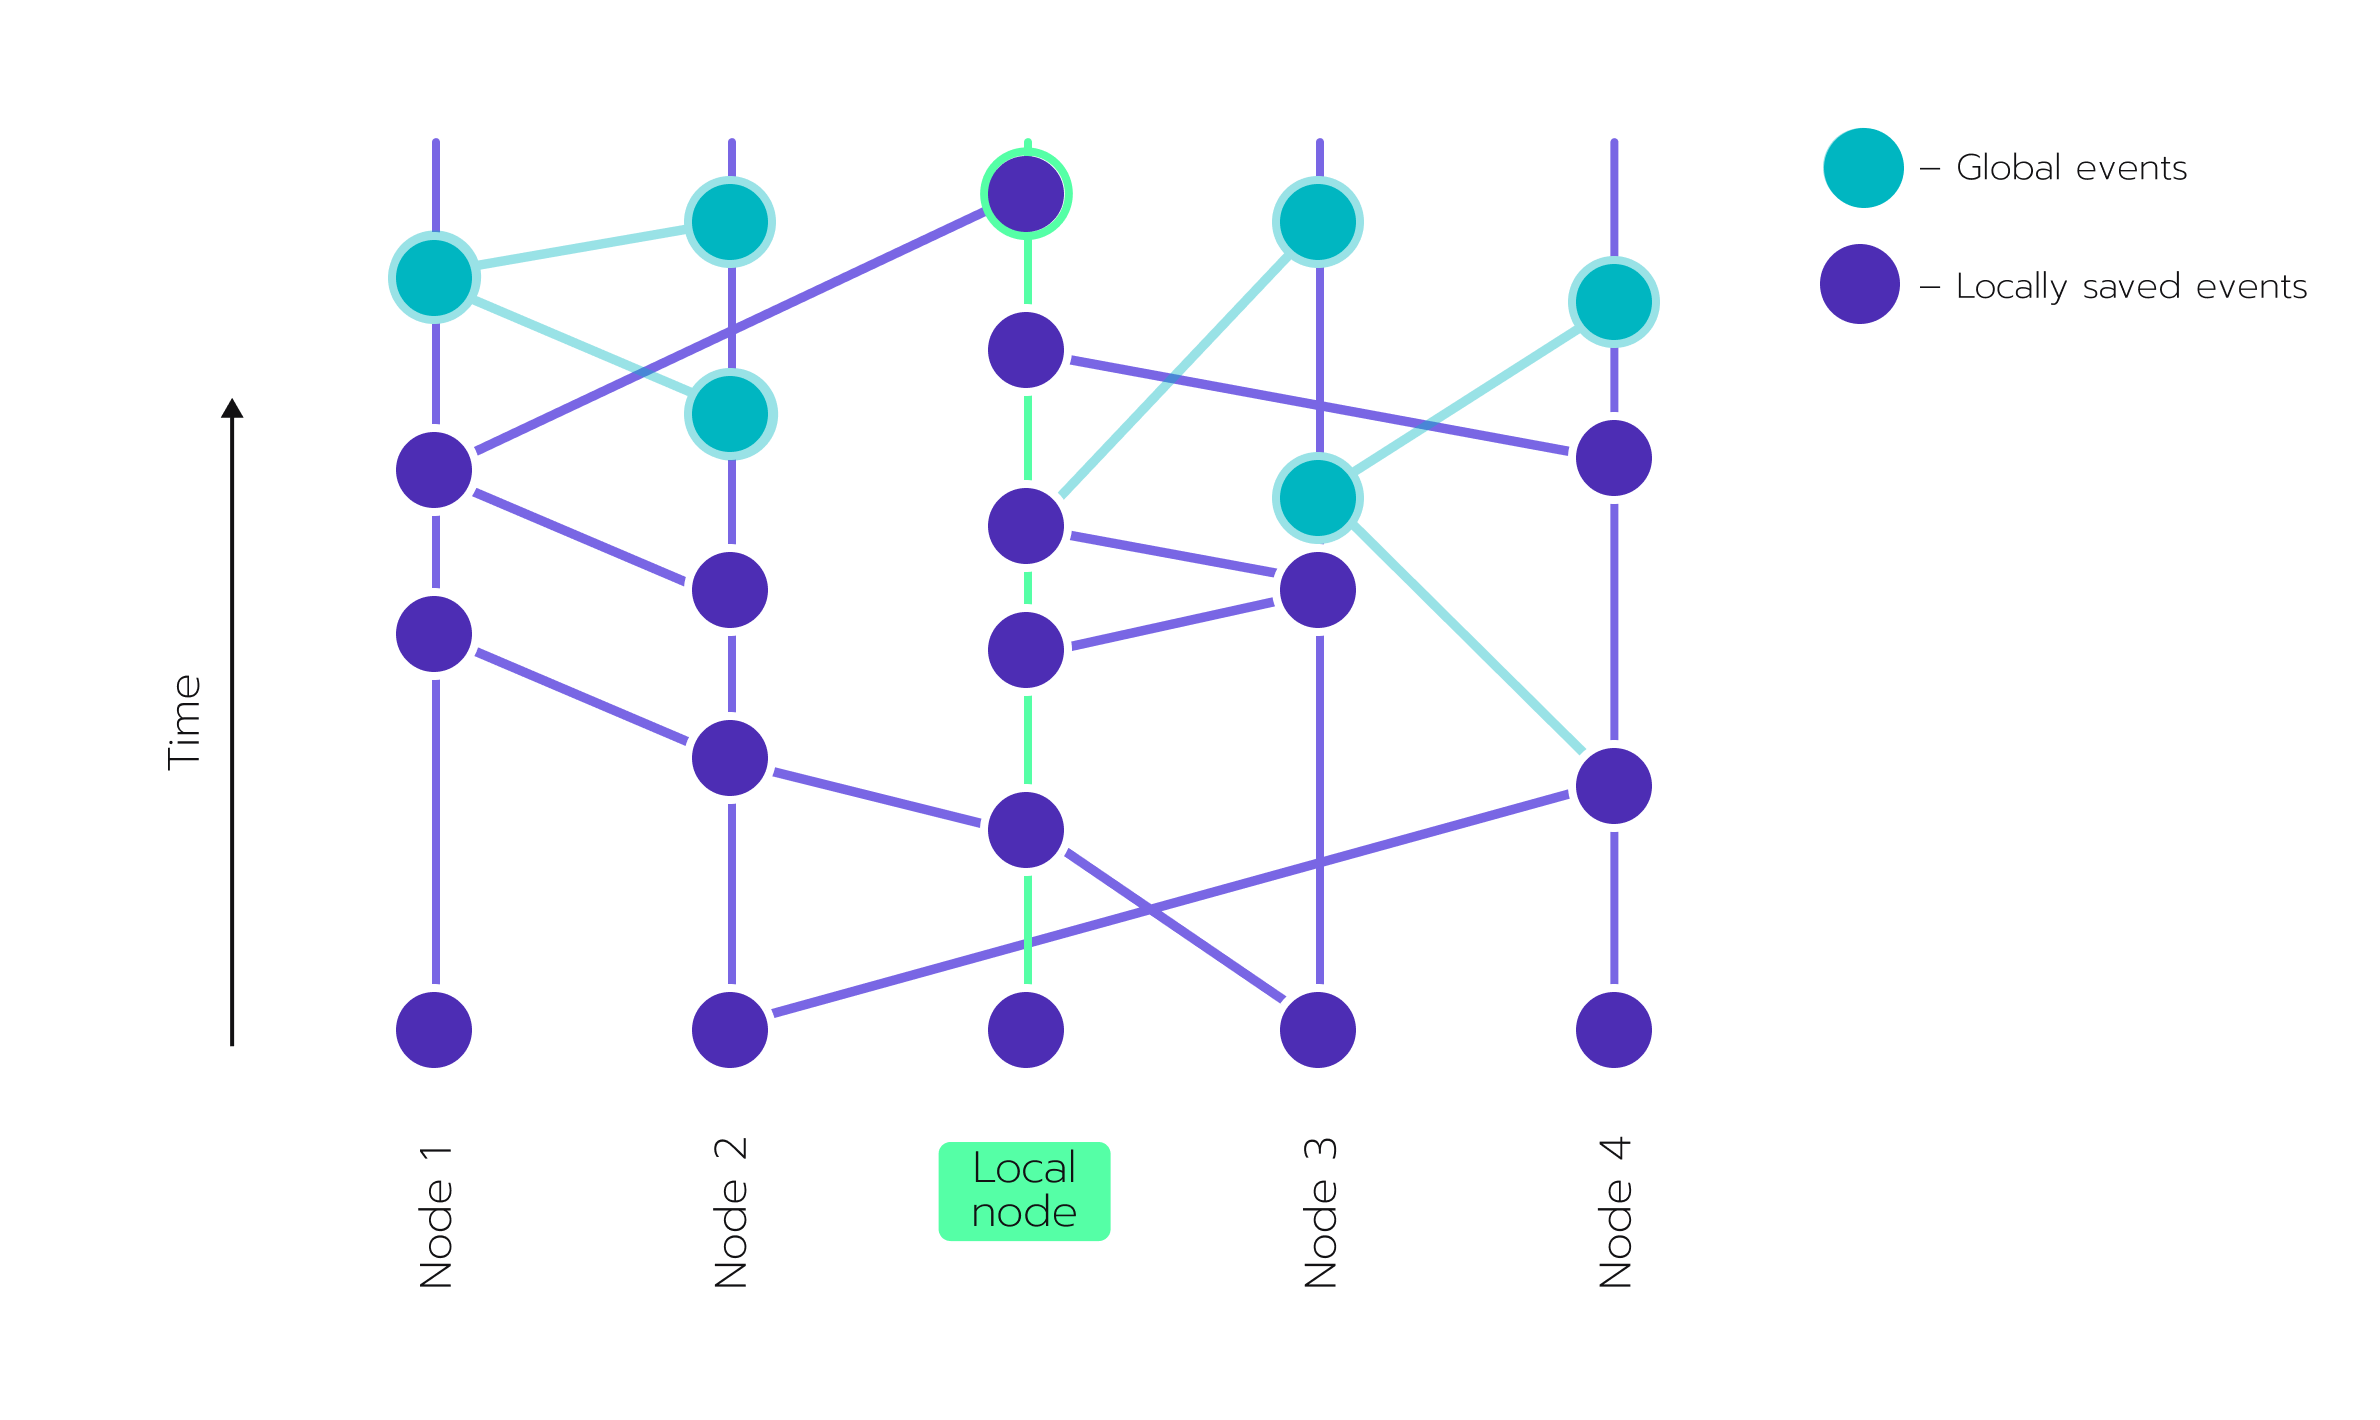
\includegraphics[width=1\textwidth]{figures/hashgraph_example.png}
        \caption{An example of the Hashgraph stored locally by a node. The transparent lines and circles represent events the local node is not \textit{yet} aware of.}
        \label{fig:hashgraph_example}
    \end{figure}

    Above is a diagram showing an example of a Hashgraph stored locally by a node. Each vertical line represents a computer node and each circle an event: Some information entering the system or being shared. The diagonal lines connecting events represent a node gossiping to another, that is, sharing the history of communication the other did not already know. It is important to note that this is not all the gossip happening in the network, just the gossip that our local computer node is aware of because other nodes have gossiped about it. The transparent lines and circles are gossip our local node is not \textit{yet} aware of because no node has gossiped the information to it. This information is not \textit{yet} saved in the local Hashgraph. So every node's local Hashgraph will differ at the top of the Hashgraph (no node is aware of all the newest gossip), but with time, all gossip will be added to every local Hashgraph.

\subsubsection{Byzantine Fault Tolerance}
    The Hashgraph consensus protocol reaches byzantine agreement on the ordering of events. This protocol is \gls{abft}, meaning that it makes no assumptions about communication delay and is tolerant of up to $\frac{1}{3}$ byzantine failures. So, even in scenarios with arbitrarily long communication delays and $\frac{1}{3}$ of the nodes sending contradictory information to disrupt the network, the system would continue to function. This makes the system very robust even under extreme circumstances which is essential in decentralised, distributed systems. A protocol where every node eventually agrees on the ordering of information is called an \acrfull{abp}. Tagion uses the original Hashgraph protocol described by Leemon Baird to reach consensus, but differs in how it implements the \gls{abp} on top. The following 2 sections describes Tagion implements a new, fairer way to order events, and a way to send information, to achieve minimal communication complexity. 

\subsection{Fair Ordering}
    Tagion uses the Hashgraph to order all information passing through the system. The Hashgraph doesn't just reach byzantine agreement on event ordering; it is constructed around how to ensure a genuinely fair ordering of events. But what is a fair ordering? A naive approach would be to say the information is ordered according to the moment the information was added to any node. This would be problematic if a node doesn't share the event for a long time: When it finally shares it the network would have to insert it in the past potentially invalidating information added since. A fairer approach is to order an event according to when the network as a whole knows of the event. The Hashgraph does this through \textit{famous witnesses}. A node is defined to become a witness
        \footnote{It is actually a specific event from a node which is defined to be a witness event. For a technically precise definition we refer to: \cite{SWIRLDS_HASHGRAPH}}
    if it is communicating actively in the network and has received messages from most of the network recently. A witness further becomes famous, if it shortly afterwards has sent messages to most of the network. A node thus both needs to talk and listen to become a famous witness. Tagion uses these famous witnesses to represent the network as a whole. If the network is running efficiently every node will be a famous witness. An event is then ordered according to the average point of when the famous witnesses first learned of this event. Abstractly, an event is ordered according to the average point that the network as a whole heard of the event. Not only does the Hashgraph order all events in the network tolerant to byzantine failures; it also does this in a fair way.
    \footnote{For a more precise and technical definition of famous, witness, and ordering we refer to our documentation and the SWIRLDS Hashgraph paper}

\subsection{The Wavefront Protocol}
    So far, we have described nodes gossiping the history of communication the other doesn't know. Sending exactly what the other doesn't know is a technically difficult task. A simple solution is to simply send all information, but this would result in much duplicate information being shared across the network. This would greatly increase the communication complexity and become a bottleneck for the system. Tagion achieves this, while maintaining a asymptotic quadratic communication complexity which is the theoretical minimum, by using its \gls{wavefront protocol}.
    
    The \gls{wavefront protocol} is used to exchange information between two nodes ensuring the minimal amount of overhead communication. Each created event has an altitude one higher than the one below it. Thus the altitude can unambiguously refer to a specific event by a certain node. Each node encodes the information it knows into a wave; the newest event it locally knows from each other node. The wavefront doesn't contain the newest information but rather numbers, the altitudes of the events representing it. By receiving the wavefront of another node you know exactly what it knows and can send just the right amount of information to the node. In the diagram below, node A and node B each have some amount of the newest gossip in their local Hashgraph. They each have a wavefront just covering all the events they locally know of. The \gls{wavefront protocol} has three states: tidal wave, first wave, and second wave.

    \begin{figure}[H]
        \centering
        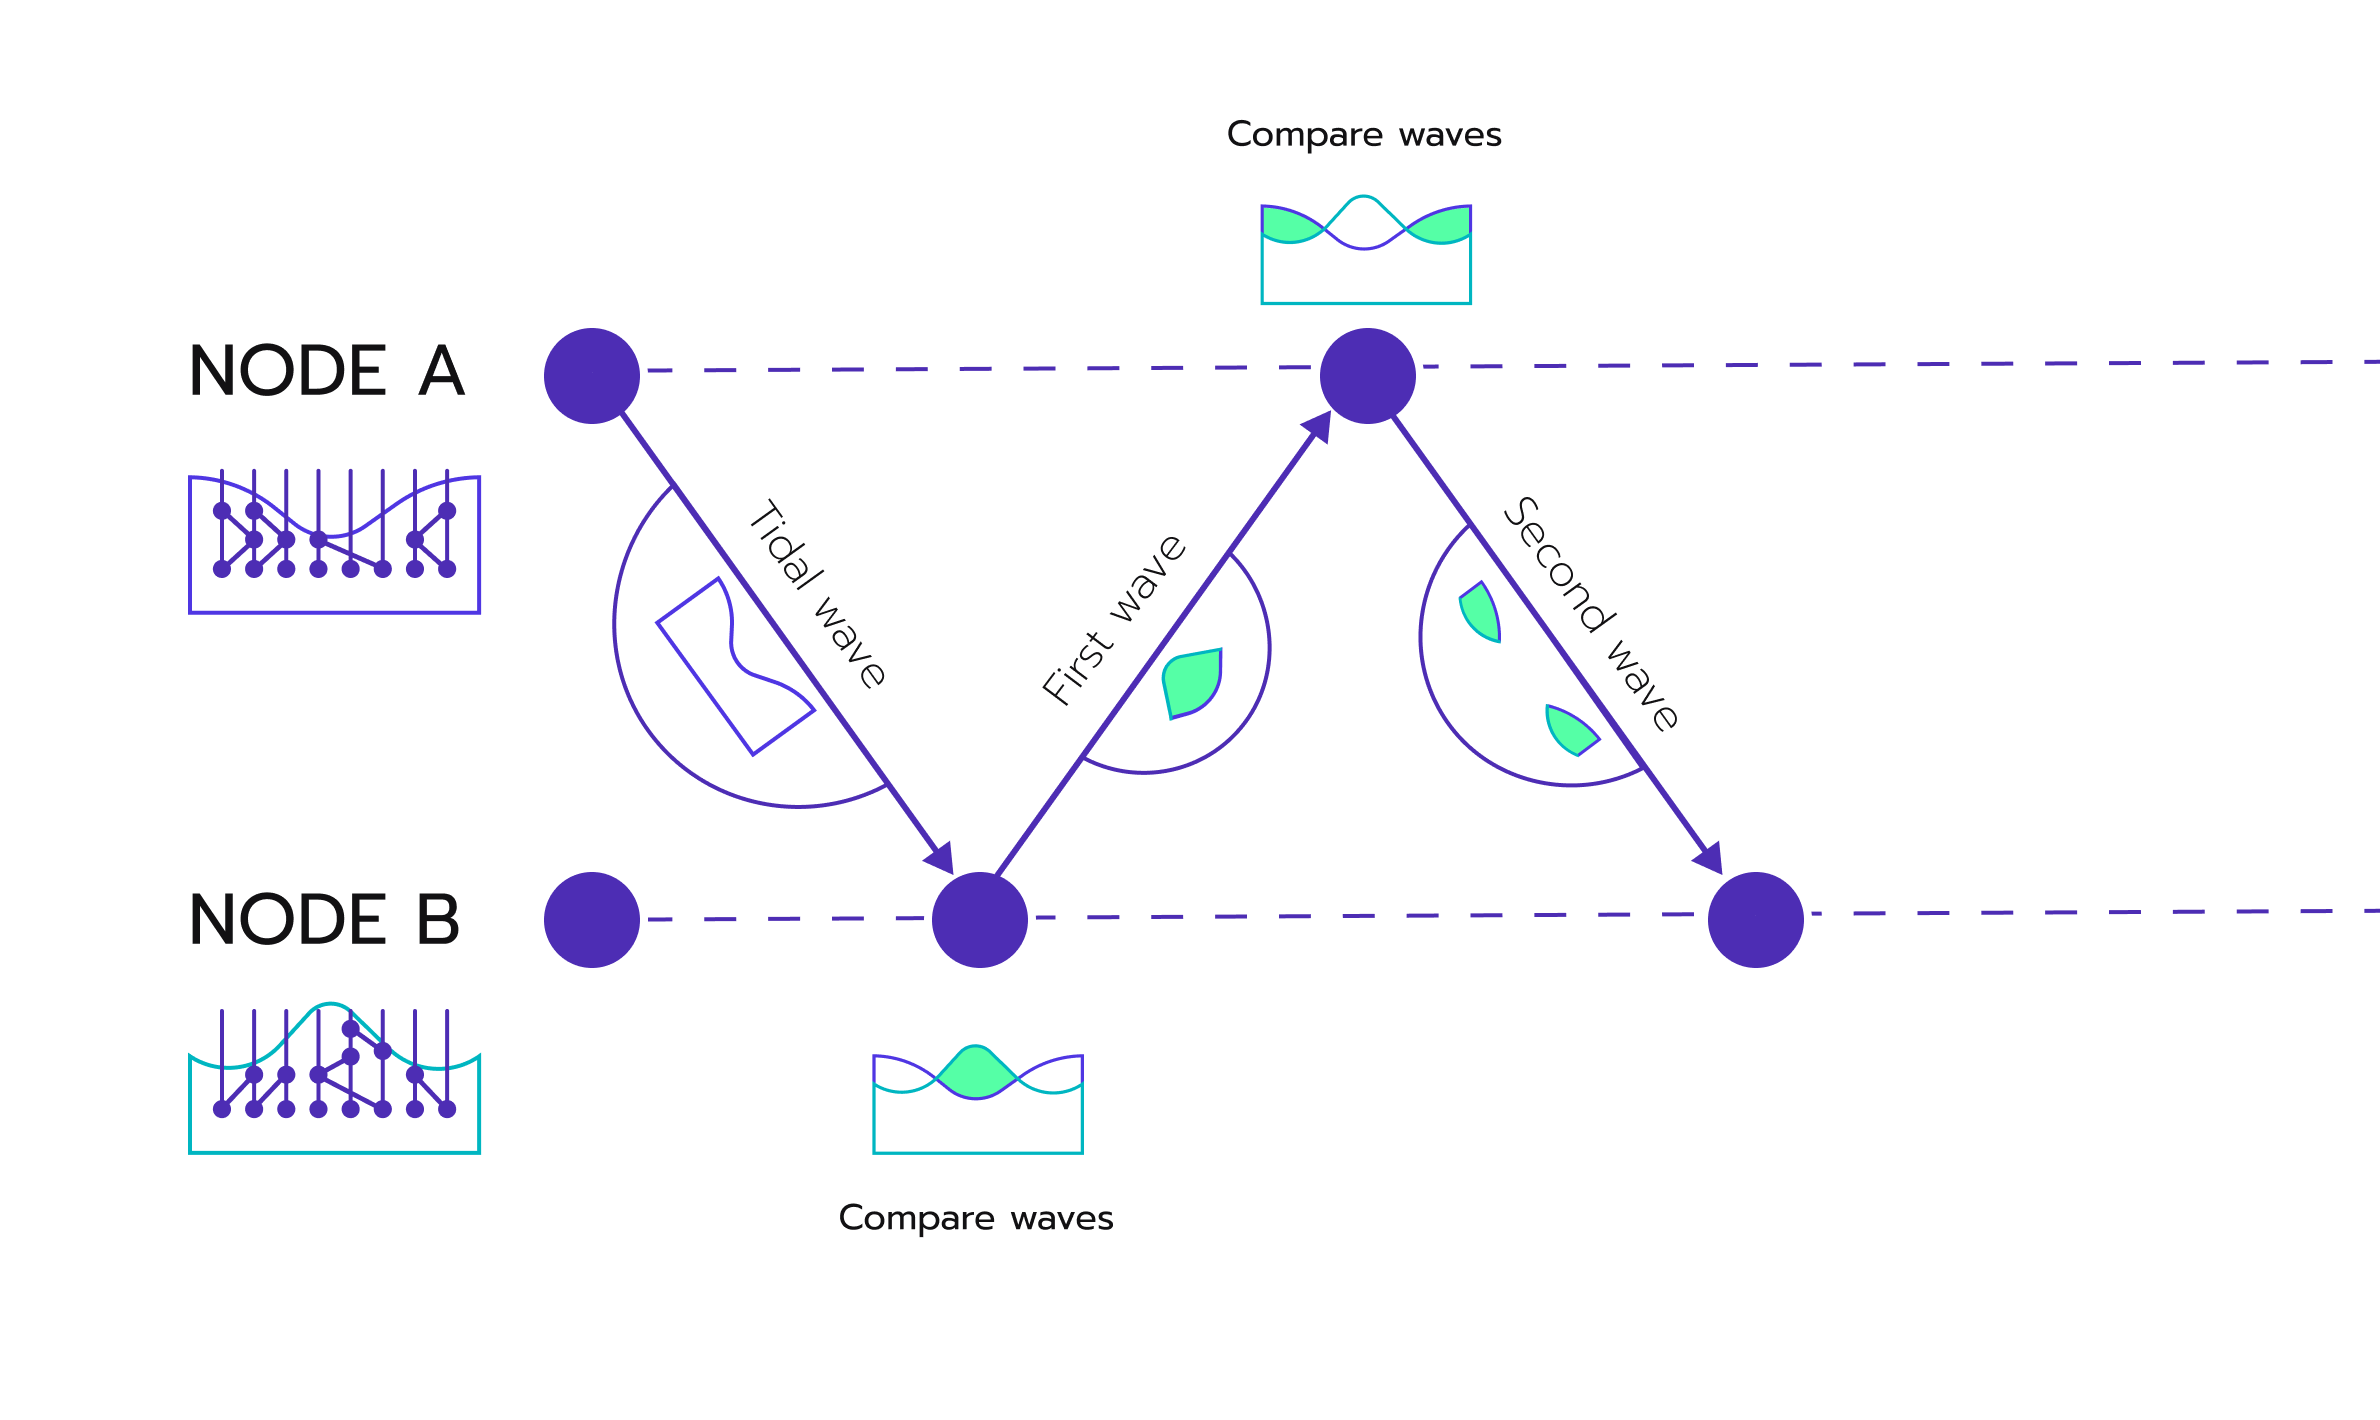
\includegraphics[width=1\textwidth]{figures/wavefront_communication.png}
    	\caption{How the \gls{wavefront protocol} works. Node A and B each has a wavefront representing what they know. By sharing and comparing their waves they can send exactly what is necessary.}
    	\label{fig:wavefront_communication}
    \end{figure}

    \begin{enumerate}
        \item Node A selects random Node B and sends its wavefront representing what it knows. This is called a tidalwave.
        \item Node B receives a tidal wave from Node A, representing exactly what A knows. Node B compares its own wavefront with the tidal wave from node A, and sends back all events which are in front of the wave of Node A; that is, tell node A exactly all information it does not know already. This is called a first wave.
        \item Node A receives a first wave from Node B and saves all the new information to its local Hashgraph. Reasoning from the information node B sent, node A can deduce the wavefront of node B. Node A then compares its own wavefront with the wavefront of node B. It then sends node B with a second wave, sending all the information node B did not know already. Node B saves all of these to its local Hashgraph.
    \end{enumerate}

\subsection{Communication Complexity}
    The \gls{wavefront protocol} allows node A and node B to share exactly what is necessary and (almost) nothing else. Since Tagion is an asynchronous system delays can cause conflicting states to occur, which is fixed by nodes sending a breaking wave resetting the states. Delays can, in theory, also cause duplicate information to be sent, but this would rarely occur in practise. The \gls{wavefront protocol} thus allows the Hashgraph protocol to be very close to the theoretically minimal communication complexity. The only overhead information that the Hashgraph shares is the tidal waves, signatures, breaking waves, and occasional duplicate information; all negligible compared to the actual information flowing through the system. As the network increases in size and throughput, the overhead becomes insignificant, achieving asymptotically optimal communication complexity. This allows Tagion to efficiently reach agreement and \textit{write} information to the system. The next section describes how Tagion efficiently \textit{reads} information from the system to achieve scalability.

\pagebreak